\caulc
\begin{ex}%[1D6H4-2]%[TDMZZ21]%%[Huynh Quốc Đạt]
	Phương trình $2^{2^x}=4^4$ có nghiệm là
	\choice
	{\True $3$}
	{$\log_2 3$}
	{$\log_2 6$}
	{$2$}
	\loigiai{
		Ta có
		\allowdisplaybreaks
		\begin{eqnarray*}
			&&2^{2^x}=4^4\\
			&\Leftrightarrow& 2^{2^x}=2^8\\
			&\Leftrightarrow& 2^x=8\\
			&\Leftrightarrow& x=3.
		\end{eqnarray*}
	}
\end{ex}

\begin{ex}%[1D6H2-1]%[TDMZZ21]%%[Huynh Quốc Đạt]
	Cho $a=\log_2 3$ và $b=\log_3 7$. Giá trị của $\log_2 14$ bằng
	\choice
	{$a+b-1$}
	{$4ab$}
	{$2ab+3$}
	{\True $ab+1$}
	\loigiai{
		Ta có
		\allowdisplaybreaks
		\begin{align*}
			\log_2 14&=\log_2 2+\log_2 7\\
			&=1+\log_2 3\cdot \log_3 7\\
			&=1+ab.
		\end{align*}
	}
\end{ex}

\begin{ex}%[1D2H3-4]%[TDMZZ21]%%[Huynh Quốc Đạt]
	Cho một cấp số nhân có tổng và tích số hạng đầu tiên và số hạng thứ tư lần lượt bằng $9$ và $8$. Tổng của số hạng thứ hai và số hạng thứ ba bằng
	\choice
	{$2\sqrt{2}$}
	{$\sqrt{13}$}
	{$4$}
	{\True $6$}
	\loigiai{
		Gọi cấp số nhân có số hạng đầu $u_1$ và công bội $q$.\\
		Ta có $\heva{&u_1+u_4=9\\&u_1\cdot u_4=8.}$\\
		Suy ra $u_1$, $u_4$ là nghiệm của phương trình
		\[X^2-9X+8=0\Leftrightarrow \hoac{&X=1\\&X=8.}\]
		Do đó $\heva{&u_1=1\\&u_4=8}$ hoặc $\heva{&u_1=8\\&u_4=1.}$\\
		Suy ra $\heva{&u_1=1\\&q=2}$ hoặc $\heva{&u_1=8\\&q=\dfrac{1}{2}.}$
		\begin{itemize}
			\item Với $u_1=1$, $q=2$.\\
			Suy ra $u_2+u_3=u_1q+u_1q^2=6$.
			\item Với $u_1=8$, $q=\dfrac{1}{2}$.\\
			Suy ra $u_2+u_3=u_1q+u_1q^2=8\cdot \dfrac{1}{2}+8\cdot\left(\dfrac{1}{2}\right)^2=6$.
		\end{itemize}
		Vậy $u_2+u_3=6$.
	}
\end{ex}

\begin{ex}%[1H8N7-2]%[TDMZZ21]%%[Huynh Quốc Đạt]
	Cho hình chóp tam giác $S. ABC$ có đáy $ABC$ là tam giác có diện tích bằng $a^2$ và cạnh bên $SA=3a$ vuông góc với mặt phẳng đáy $(ABC)$. Thể tích của hình chóp $S. ABC$ bằng
	\choice
	{$9a^3$}
	{$3a^3$}
	{\True $a^3$}
	{$2a^3$}
	\loigiai{
		\immini{Ta có $V_{S. ABC}=\dfrac{1}{3}\cdot SA\cdot S_{\triangle ABC}=\dfrac{1}{3}\cdot 3a\cdot a^2=a^3$.}
		{\begin{tikzpicture}[>=stealth,scale=0.7, font=\footnotesize, line join=round,line cap=round]
				\coordinate (A) at (-2,0);
				\coordinate (B) at (0,-3);
				\coordinate (C) at (3,0);
				\coordinate (S) at ($(A)+(0,4)$);
				\draw(S)--(A) (S)--(B) (S)--(C) (B)--(C) (A)--(B);
				\draw[dashed,thin](A)--(C);
				\pic[draw,thin,angle radius=2mm] {right angle = S--A--B} pic[draw,thin,angle radius=2mm] {right angle = S--A--C};
				\foreach \i/\g in {S/90,A/180,B/-90,C/0}{\draw[fill=black](\i) circle (1pt) ($(\i)+(\g:3mm)$) node[scale=1]{$\i$};}
		\end{tikzpicture}}
	}
\end{ex}

\begin{ex}%[2D1N1-2]%[TDMZZ21]%%[Huynh Quốc Đạt]
	Cho hàm số $f(x)$ có bảng biến thiên như hình vẽ bên dưới
	\begin{center}
		
\begin{tikzpicture}
			\tkzTabInit[nocadre=false,lgt=1,espcl=2,deltacl=0.5]
			{$x$/0.7,$f(x)$/2}{$-\infty$,$-4$,$0$,$3$,$+\infty$}
			\tkzTabVar{-/$-\infty$,+/$4$,-/$-2$,+/$3$,-/$-\infty$}
		\end{tikzpicture}
	\end{center}
	Hỏi hàm số nghịch biến trên khoảng nào dưới đây?
	\choice
	{$(-\infty;-1)$}
	{$(1;2)$}
	{\True $(3;+\infty)$}
	{$(-4;1)$}
	\loigiai{
		Dựa vào bảng biến thiên, hàm số nghịch biến trên các khoảng $(-4;0)$ và $(3;+\infty)$.
	}
\end{ex}

\begin{ex}%[2D4N2-2]%[TDMZZ21]%%[Huynh Quốc Đạt]
	Giá trị của tích phân $\displaystyle\int\limits_{0}^{1}2x\mathrm{\,d}x$ bằng
	\choice
	{\True $1$}
	{$2$}
	{$4$}
	{$0$}
	\loigiai{
		Ta có $\displaystyle\int\limits_{0}^{1}2x\mathrm{\,d}x=x^2\Bigg|^1_0=1^2=1$.
	}
\end{ex}

\begin{ex}%[2H5N1-2]%[TDMZZ21]%%[Huynh Quốc Đạt]
	Trong không gian $Oxyz$, cho mặt phẳng $(P)\colon x-2y+3z+1=0$. Hỏi vectơ nào dưới đây là một vectơ pháp tuyến của mặt phẳng $(P)$?
	\choice
	{\True $(1;-2;3)$}
	{$(1;2;3)$}
	{$(-2;3;1)$}
	{$(2;-2;4)$}
	\loigiai{
		Ta có $(P)\colon x-2y+3z+1=0$ suy ra một vectơ pháp tuyến của mặt phẳng $(P)$ là $\overrightarrow{n}=(1;-2;3)$.
	}
\end{ex}

\begin{ex}%[2D1N4-1]%[TDMZZ21]%%[Huynh Quốc Đạt]
	Số đường tiệm cận của đồ thị của hàm số $y=\dfrac{x+2}{x-1}$ là
	\choice
	{$1$}
	{\True $2$}
	{$3$}
	{$0$}
	\loigiai{
		Ta có $\lim\limits_{x\to 1^+}\dfrac{x+2}{x-1}=+\infty$ và $\lim\limits_{x\to 1^-}\dfrac{x+2}{x-1}=-\infty$.\\
		Suy ra $x=1$ là tiệm cận đứng của đồ thị hàm số.\\
		Lại có $\lim\limits_{x\to\pm\infty}\dfrac{x+2}{x-1}=1$ nên $y=1$ là tiệm cận ngang của đồ thị hàm số.\\
		Vậy đồ thị có $2$ đường tiệm cận.
	}
\end{ex}

\begin{ex}%[2H5N3-2]%[TDMZZ21]%%[Huynh Quốc Đạt]
	Trong không gian $Oxyz$, cho mặt cầu $(S)\colon x^2+y^2+z^2-4x-5=0$. Tâm mặt cầu có toạ độ là
	\choice
	{$(0;0;-1)$}
	{$(0;0;1)$}
	{\True $(2;0;0)$}
	{$(0;0;-2)$}
	\loigiai{
		Ta có $\heva{&a=\dfrac{-4}{-2}=0\\&b=\dfrac{0}{-2}=0\\&c=\dfrac{0}{-2}=0}\Leftrightarrow\heva{&a=2\\&b=0\\&c=0.}$\\
		Suy ra mặt cầu $(S)$ có tâm $I(2;0;0)$.\\
		Bán kính $R=\sqrt{a^2+b^2+c^2-d}=\sqrt{2^2+0^2+0^2-(-5)}=3$.
	}
\end{ex}

\begin{ex}%[2D4N3-1]%[TDMZZ21]%%[Huynh Quốc Đạt]
	\immini[thm]{Diện tích phần gạch chéo ở hình vẽ được tính theo công thức tương ứng là
		\choice
		{$S=\displaystyle\int\limits_{-2}^{3}f(x)\mathrm{\,d}x$}
		{$S=\left|\displaystyle\int\limits_{-2}^{3}f(x)\mathrm{\,d}x\right|$}
		{$S=-\displaystyle\int\limits_{-2}^{1}f(x)\mathrm{\,d}x+\displaystyle\int\limits_{1}^{3}f(x)\mathrm{\,d}x$}
		{\True $S=\displaystyle\int\limits_{-2}^{1}f(x)\mathrm{\,d}x-\displaystyle\int\limits_{1}^{3}f(x)\mathrm{\,d}x$}}
	{	\begin{tikzpicture}[>=stealth,scale=0.7, font=\footnotesize, line join=round,line cap=round]
			\def\xmin{-3} \def\xmax{4}
			\def\ymin{-3} \def\ymax{4}
			\draw[->] (\xmin,0)--(0,0)node[below left]{$O$}--(\xmax,0) node[below]{$x$};
			\draw[->] (0,\ymin)--(0,\ymax)node[right]{$y$};
			\path (-2,0) coordinate (A) (1,0) coordinate (B) (3,0) coordinate (C);
			\fill (A) circle (1.2pt) node[below right]{$-2$};
			\fill (B) circle (1.2pt) node[above right]{$1$};
			\fill (C) circle (1.2pt) node[below right]{$3$};
			\begin{scope}
				\clip (\xmin,\ymin) rectangle (\xmax,\ymax);
				\draw[smooth,samples=120,domain=\xmin:\xmax,thick] plot(\x,{0.3*(\x+2)*(\x-1)*(\x-3)});
			\end{scope}
			\begin{scope}
				\clip plot[smooth,samples=120,domain=-2:1](\x,{0.3*(\x+2)*(\x-1)*(\x-3)})--(1,0)--(-2,0)--cycle;
				\fill[pattern=north east lines] (\xmin,\ymin) rectangle (\xmax,\ymax);
			\end{scope}
			\begin{scope}
				\clip plot[smooth,samples=120,domain=1:3](\x,{0.3*(\x+2)*(\x-1)*(\x-3)})--(3,0)--(1,0)--cycle;
				\fill[pattern=north east lines] (\xmin,\ymin) rectangle (\xmax,\ymax);
			\end{scope}
			\path (2.2,3) node[right]{$f(x)$};
	\end{tikzpicture}}
	\loigiai{
		Trên đoạn $[-2;1]$, đồ thị nằm phía trên trục hoành nên $f(x)\ge 0$.\\
		Trên đoạn $[1;3]$, đồ thị nằm phía dưới trục hoành nên $f(x)\le 0$.\\
		Do đó $S=\displaystyle\int\limits_{-2}^{1}f(x)\mathrm{\,d}x-\displaystyle\int\limits_{1}^{3}f(x)\mathrm{\,d}x$.
	}
\end{ex}

\begin{ex}%[2H2H1-2]%[TDMZZ21]%%[Huynh Quốc Đạt]
	Cho hình chóp tứ giác đều $S. ABCD$. Gọi $O$ là điểm thoả mãn hệ thức vectơ \break $\overrightarrow{SA}+\overrightarrow{SB}+\overrightarrow{SC}+\overrightarrow{SD}=2\overrightarrow{SO}$. Nhận xét đúng về điểm $O$ là
	\choice
	{$O$ đối xứng với $A$ qua $C$}
	{$SBOD$ là hình vuông}
	{\True $SAOC$ là hình bình hành}
	{$ACOD$ là hình bình hành}
	\loigiai{
		\immini{Gọi $I$ là tâm hình vuông $ABCD$.\\
			Ta có $\overrightarrow{SA}+\overrightarrow{SC}=2\overrightarrow{SI}$ và $\overrightarrow{SB}+\overrightarrow{SD}=2\overrightarrow{SI}$.\\
			Do đó $\overrightarrow{SA}+\overrightarrow{SB}+\overrightarrow{SC}+\overrightarrow{SD}=4\overrightarrow{SI}=2\overrightarrow{SO}$ nên $\overrightarrow{SO}=2\overrightarrow{SI}$, tức là $I$ là trung điểm của $SO$.\\
			Mà $I$ cũng là trung điểm của $AC$ nên $SAOC$ là hình bình hành.}
		{\begin{tikzpicture}[>=stealth,scale=0.7, font=\footnotesize, line join=round,line cap=round]
				\coordinate (A) at (0,0);
				\coordinate (B) at (2,-2);
				\coordinate (D) at (5,0);
				\coordinate (C) at ($(B)+(D)-(A)$);
				\coordinate (I) at ($(A)!0.5!(C)$);
				\coordinate (S) at ($(I)+(0,5)$);
				\coordinate (O) at ($(S)!2!(I)$);
				\draw(S)--(A)--(O)--(C) (S)--(B) (S)--(C) (A)--(B) (B)--(C);
				\draw[dashed](A)--(C) (A)--(D) (C)--(D) (S)--(D) (S)--(I) (B)--(D);
				\foreach \i/\g in {S/90,A/180,B/-90,C/-90,D/0,I/-90,O/0}{\draw[fill=black](\i) circle (1pt) ($(\i)+(\g:3mm)$) node[scale=1]{$\i$};}
		\end{tikzpicture}}
	}
\end{ex}

\begin{ex}%[2D3V1-2]%[TDMZZ21]%%[Huynh Quốc Đạt]
	Cho mẫu số liệu ghép nhóm $M$ có tất cả $8$ nhóm với độ dài bằng nhau. Biết rằng đầu mút phải của nhóm thứ $n$ có giá trị bằng đầu mút trái của nhóm thứ $n+1$, đầu mút trái của nhóm thứ $6$ nhiều hơn phần tử đại diện của nhóm thứ $2$ là $14$ đơn vị. Hãy xác định khoảng biến thiên của mẫu số liệu $M$?
	\choice
	{$28$}
	{$56$}
	{\True $32$}
	{$42$}
	\loigiai{
		Gọi đầu mút trái của nhóm thứ nhất là $a$ và độ dài mỗi nhóm là $h$.\\
		Đầu mút trái của nhóm thứ $6$ là $a+5h$.\\
		Phần tử đại diện của nhóm thứ $2$ là $a+\dfrac{3h}{2}$.\\
		Theo giả thiết $(a+5h)-\left(a+\dfrac{3h}{2}\right)=14\Leftrightarrow \dfrac{7h}{2}=14\Leftrightarrow h=4$.\\
		Khoảng biến thiên của mẫu số liệu là $R=8h=8\cdot 4=32$.
	}
\end{ex}
\cauds
\begin{ex}%[2D1V2-5]%[Dương Công Tạo]
	Trong mặt phẳng toạ độ $Oxy$, cho hàm số $y = f(x) = x^4 - 4x^2 + 3$ có đồ thị $(C)$.
	\choiceTF
	{$f'(x) = 4x^3 - 4x$}
	{\True Ba điểm cực trị của $(C)$ tạo thành một tam giác cân}
	{Diện tích của tam giác tạo bởi ba điểm cực trị của $(C)$ bằng $4$}
	{Ba điểm cực trị của $(C)$ tạo thành một tam giác có bán kính đường tròn ngoại tiếp bằng $2$}
	\loigiai{
		\begin{itemchoice}
			\itemch Xét hàm số $y = f(x) = x^4 - 4x^2 + 3$ trên khoảng $\left(-\infty;+\infty\right)$.\\
			Ta có $f'(x) = 4x^3 - 8x=4x\left(x^2-2\right)$.
			\itemch $f'(x) =0\Leftrightarrow \hoac{&x=0\\&x=\pm\sqrt{2}.}$\\
			Bảng biến thiên
			\begin{center}
				
\begin{tikzpicture}[>=stealth]
					\tkzTabInit[nocadre=false,lgt=1.5,espcl=2,deltacl=0.6]{$x$/.7 ,$f'(x)$/.7,$f(x)$/2}
					{$-\infty$ , $-\sqrt{2}$ , $0$ , $\sqrt{2}$ , $+\infty$}
					\tkzTabLine{ , - , 0 , + , 0 , - , 0 , + , }
					\tkzTabVar{+/$+\infty$ , -/$-1$ , +/$3$ ,-/$-1$ , +/$+\infty$}
				\end{tikzpicture}
			\end{center}
			Suy ra, đồ thị hàm số đạt cực trị tại ba điểm $A(0;3)$, $B\left(-\sqrt{2};-1\right)$ và $C\left(\sqrt{2};-1\right)$.\\
			Mà $AB=AC=\sqrt{\left(\sqrt{2}-0\right)^2+(-1-3)^2}=3\sqrt{2}$ nên $\triangle ABC$ cân tại $A$.
			\itemch Gọi $H(0;-1)$ là trung điểm của $BC$ thì $AH\perp BC$ vì $\triangle ABC$ cân tại $A$.\\
			Khi đó, diện tích $\triangle ABC$ là $S_{ABC}=\dfrac{1}{2}\cdot AH\cdot BC=\dfrac{1}{2}\cdot4\cdot2\sqrt{2}=4\sqrt{2}$.
			\itemch Ta có $S_{ABC}=\dfrac{AB\cdot AC\cdot BC}{4R}\Rightarrow R=\dfrac{AB\cdot AC\cdot BC}{4S}=\dfrac{3\sqrt{2}\cdot 3\sqrt{2}\cdot 2\sqrt{2}}{4\cdot4\sqrt{2}}=\dfrac{9}{4}$.
		\end{itemchoice}
	}
\end{ex}

\begin{ex}%[TDMZZ21]%[Hà Văn Hảo]%[2H5V3-2]
	Trong không gian $Oxyz$, cho mặt cầu $(S) \colon x^2 + (y - 1)^2 + (z - 2)^2 = 15$ và điểm $A(2; -3; -2)$. Gọi $M$ và $N$ là hai điểm thay đổi chạy trên $(S)$ sao cho ba điểm $A$, $M$, $N$ thẳng hàng.
	\choiceTF
	{\True Tâm của mặt cầu $(S)$ là $I(0; 1; 2)$ và bán kính của $(S)$ là $R = \sqrt{15}$}
	{\True $A$ nằm ngoài mặt cầu $(S)$}
	{\True $AM \cdot AN = 21$}
	{Giá trị nhỏ nhất của biểu thức $AM + 2AN$ bằng $12$}
	\loigiai{
		\begin{itemchoice}
			\itemch Từ phương trình mặt cầu $(S) \colon x^2 + (y - 1)^2 + (z - 2)^2 = 15$, ta xác định được tâm $I(0; 1; 2)$ và bán kính $R = \sqrt{15}$.
			\itemch Ta tính khoảng cách từ $A$ đến tâm $I$
			$$IA = \sqrt{(2 - 0)^2 + (-3 - 1)^2 + (-2 - 2)^2} = \sqrt{4 + 16 + 16} = \sqrt{36} = 6$$
			Vì $IA = 6 > R = \sqrt{15}$ nên điểm $A$ nằm ngoài mặt cầu $(S)$.
			\itemch Vì $A$, $M$, $N$ thẳng hàng và $M$, $N$ thuộc mặt cầu $(S)$, nên tích $AM \cdot AN$ chính là trị tuyệt đối của phương tích của điểm $A$ đối với mặt cầu $(S)$
			\[AM \cdot AN = |IA^2 - R^2| = |6^2 - (\sqrt{15})^2| = |36 - 15| = 21.\]
			\itemch Đặt $AM = x$ và $AN = y$ ($x, y > 0$). Theo kết quả câu c, ta có $xy = 21$.\\
			Biểu thức cần tìm giá trị nhỏ nhất là $P = x + 2y$.\\
			Áp dụng bất đẳng thức AM-GM (Cauchy) cho hai số dương $x$ và $2y$
			\[P = x + 2y \ge 2\sqrt{x \cdot 2y} = 2\sqrt{2xy} = 2\sqrt{2 \cdot 21} = 2\sqrt{42} \approx 12{,}96.\]
			Tuy nhiên, cần lưu ý rằng $M$, $N$ là giao điểm của đường thẳng đi qua $A$ với mặt cầu. Độ dài đoạn thẳng $MN = |x - y|$ phải thỏa mãn điều kiện dây cung $MN \le 2R = 2\sqrt{15}$.\\
			Đoạn thẳng $AM$ và $AN$ có giá trị nằm trong đoạn $[IA - R; IA + R]$, tức là $[6 - \sqrt{15}; 6 + \sqrt{15}]$.\\
			Xét hàm số $f(y) = \dfrac{21}{y} + 2y$ trên đoạn $[6 - \sqrt{15}; 6 + \sqrt{15}]$.\\
			$f'(y) = -\dfrac{21}{y^2} + 2$. Cho $f'(y) = 0 \Leftrightarrow y^2 = \dfrac{21}{2} = 10{,}5 \Rightarrow y = \sqrt{10{,}5} \approx 3{,}24$.\\
			Giá trị $y = \sqrt{10{,}5}$ nằm trong khoảng $[6 - \sqrt{15}; 6 + \sqrt{15}] \approx [2{,}13; 9{,}87]$.\\
			Vậy giá trị nhỏ nhất là $P_{\min} = 2\sqrt{42} \approx 12{,}96$.
		\end{itemchoice}
	}
\end{ex}

\begin{ex}%[2D6V2-4]%[TDMZZ21]%[Vũ Hồng Toàn]
	Theo thống kê thì: tỉ lệ học sinh học tốt và chăm chỉ lao động sẽ có thu nhập cao trong tương lai là $90\%$, còn lại thì sẽ có thu nhập cao trong tương lai là $20\%$. Bình thường thì cũng rất ít người vừa học tốt vừa chăm chỉ, thống kê trong $200$ người thì chỉ có được $10$ người vừa học tốt vừa chăm chỉ. Chọn ngẫu nhiên từ $200$ người này ra một người. Gọi $A$ là biến cố chọn được người vừa học tốt vừa chăm chỉ, $B$ là biến cố chọn được người sẽ có thu nhập cao trong tương lai.
	\choiceTF
	{\True $\mathrm{P}(A)=0{,}05$, $\mathrm{P}\left(\overline{A}\right)=0{,}95$}
	{\True $\mathrm{P}(B\mid A)=0{,}9$}
	{\True $\mathrm{P}(A\mid B)=\dfrac{9}{47}$}
	{\True Trong những người có thu nhập cao phần lớn không phải là những người vừa học tốt và vừa chăm chỉ}
	\loigiai{
		\begin{itemchoice}
			\itemch Số phần tử của không gian mẫu là $n(\Omega) =\mathrm{C}_{200}^{1}=200$.\\
			Số người vừa học tốt vừa chăm chỉ là $10$ người nên $n(A)=10$.\\
			Vậy, xác suất chọn được người vừa học tốt vừa chăm chỉ là
			\[\mathrm{P}(A) = \dfrac{n(A)}{n(\Omega)}=\dfrac{10}{200} = 0{,}05.\]
			Suy ra $\mathrm{P}\left(\overline{A}\right) = 1 - \mathrm{P}(A) = 1 - 0{,}05 = 0{,}95$.
			\itemch Vì tỉ lệ người vừa học tốt vừa chăm chỉ có thu nhập cao trong tương lai là $90\%$ nên \[\mathrm{P}(B\mid A) = 90\% = 0{,}9.\]
			\itemch Tỉ lệ những người còn lại (không đồng thời học tốt và chăm chỉ) có thu nhập cao trong tương lai là $20\%$, do đó
			$\mathrm{P}\left(B|\overline{A}\right) = 20\% = 0{,}2$.\\
			Áp dụng công thức xác suất toàn phần, ta có xác suất chọn được người có thu nhập cao trong tương lai là
			\begin{eqnarray*}
				\mathrm{P}(B) &=& \mathrm{P}(A) \cdot \mathrm{P}(B\mid A) + \mathrm{P}\left(\overline{A}\right) \cdot \mathrm{P}\left(B\mid \overline{A}\right) \\
				&=& 0{,}05 \cdot 0{,}9 + 0{,}95 \cdot 0{,}2 = 0{,}235.
			\end{eqnarray*}
			Áp dụng công thức Bayes, xác suất để người có thu nhập cao là người vừa học tốt vừa chăm chỉ là
			\[\mathrm{P}(A\mid B) = \dfrac{\mathrm{P}(A) \cdot \mathrm{P}(B\mid A)}{\mathrm{P}(B)} = \dfrac{0{,}05 \cdot 0{,}9}{0{,}235} = \dfrac{9}{47}.\]
			\itemch Xác suất để một người có thu nhập cao không phải là người vừa học tốt và vừa chăm chỉ là
			\[\mathrm{P}\left(\overline{A}\mid B\right) = 1 - \mathrm{P}(A\mid B) = 1 - \dfrac{9}{47} \approx 80{,}85\%.\]
			Vì $80{,}85\% > 50\%$ nên trong những người có thu nhập cao, phần lớn không phải là những người vừa học tốt và vừa chăm chỉ.
		\end{itemchoice}
	}
\end{ex}

\begin{ex}%[2D4V3-1]%[TDMZZ21]%[Văn Minh Thoại]
	\immini[thm]{
		Trong mặt phẳng $Oxy$, cho hình phẳng $(H)$ giới hạn bởi các đường $y=x+2$, $y=x-2$, $y=\dfrac{1}{x}$ được tô màu, cho hình phẳng $\left(H_1\right)$ được gạch chéo, cho các điểm $A$, $B$, $C$, $D$ như hình vẽ
		\choiceTF
		{\True $A\left(-1-\sqrt{2}; 1-\sqrt{2}\right)$, $B\left(-1+\sqrt{2}; 1+\sqrt{2}\right)$}
		{$C\left(1-\sqrt{2}; -1-\sqrt{2}\right)$, $D\left(1+\sqrt{2}; -1+\sqrt{2}\right)$}
		{\True Diện tích $\left(H_1\right)$ là $1{,}07$ cm$^2$ \textit{(làm tròn kết quả đến hàng phần trăm)}}
		{\True Diện tích $(H)$ là $9{,}18$ cm$^2$ \textit{(làm tròn kết quả đến hàng phần trăm)}}
	}{
		\begin{tikzpicture}[declare function={f (\x) = \x + 2; g (\x) = \x - 2; h (\x) = 1/\x; lineBC (\x) = -\x + 2*sqrt (2); xA =-1-sqrt (2); yA = 1 - sqrt (2); xB = -1 + sqrt (2); xmin = -3.5; xmax = 4.5; ymin = -3.5; ymax = 3.5;},line join=round,line cap=round,>=stealth,scale=1]
			\path
			(0,0) coordinate (O)
			({-1-sqrt (2)},{1-sqrt (2)}) coordinate (A)
			({-1 + sqrt (2)},{1 + sqrt (2)}) coordinate (B)
			({1 + sqrt (2)},{-1 + sqrt (2)}) coordinate (C)
			({1 - sqrt (2)},{-1 - sqrt (2)}) coordinate (D);		
			\begin{scope}
				\clip (xmin,ymin) rectangle (xmax,ymax);
				\fill[olive!15]
				(A) -- (B)
				-- plot[domain=0.4142:2.4142,smooth,samples=100] (\x,{h (\x)})
				-- (D)
				-- plot[domain=-0.4142:-2.4142,smooth,samples=100] (\x,{h (\x)})
				-- cycle;
				\fill[pattern = {Lines[distance=2pt,angle=45]},pattern color = red]
				plot[domain=0.4142:2.4142,smooth,samples=100] (\x,{h (\x)})
				-- (B) -- cycle;
			\end{scope}
			\draw[->] (xmin,0) -- (xmax,0) node[below] {$x$};
			\draw[->] (0,ymin) -- (0,ymax) node[shift={(-6pt,-5pt)}] {$y$};
			\begin{scope}
				\clip (xmin,ymin) rectangle (xmax,ymax);
				\draw[blue,smooth,samples=150,domain=-3.5:-0.25] plot (\x,{h (\x)});
				\draw[blue,smooth,samples=150,domain=0.25:4.5] plot (\x,{h (\x)});
				\draw[smooth,domain=-3.5:4.5] plot (\x,{f (\x)});
				\draw[smooth,domain=-3.5:4.5] plot (\x,{g (\x)});
				\draw[red,smooth,domain=-0.5:4] plot (\x,{lineBC (\x)});
			\end{scope}
			\draw[dashed,fill] (A) -- ({-1-sqrt (2)},0) circle (1pt)
			(D) -- ({1 - sqrt (2)},0) circle (1pt)
			(B) -- ({-1 + sqrt (2)},0) circle (1pt)
			(C) -- ({1 + sqrt (2)},0) circle (1pt);		
			\foreach \t/\g in {B/0,C/90,A/-90,D/180,O/-45}{
				\fill[ball color=red] (\t) circle (1pt) node[shift={(\g:9pt)},font = \footnotesize]{$\t$};
			}
			\node at (-0.6,0.6) {$(H)$};
			\draw[<-] (1.4,1)--($(C)+(0.5,2)$) node[above] {$(H_1)$};		
		\end{tikzpicture}
	}
	\loigiai{
		\begin{itemchoice}
			\itemch Xét phương trình hoành độ giao điểm của đường thẳng $y = x+2$ và đường cong $(C) \colon y = \dfrac{1}{x}$, khi đó
			\[ x + 2 = \dfrac{1}{x} \Leftrightarrow x^2 + 2x - 1 = 0 \Leftrightarrow\hoac{&x = -1 - \sqrt{2} \Rightarrow y = 1 - \sqrt{2} \\ &x = -1 + \sqrt{2} \Rightarrow y = 1 + \sqrt{2}.} \]
			Dựa vào vị trí các điểm trên đồ thị, ta có $A\left(-1-\sqrt{2}; 1-\sqrt{2}\right)$ và $B\left(-1+\sqrt{2}; 1+\sqrt{2}\right)$.
			
			\itemch Xét phương trình hoành độ giao điểm của đường thẳng $y = x-2$ và đường cong $(C) \colon y = \dfrac{1}{x}$, khi đó
			\[ x - 2 = \dfrac{1}{x} \Leftrightarrow x^2 - 2x - 1 = 0 \Leftrightarrow\hoac{&x = 1 - \sqrt{2} \Rightarrow y = -1 - \sqrt{2} \\& x = 1 + \sqrt{2} \Rightarrow y = -1 + \sqrt{2}. }\]
			Dựa vào đồ thị, điểm $C$ có hoành độ dương và điểm $D$ có hoành độ âm. \\
			Suy ra $C\left(1+\sqrt{2}; -1+\sqrt{2}\right)$ và $D\left(1-\sqrt{2}; -1-\sqrt{2}\right)$.
			
			\itemch Giả sử phương trình đường thẳng $BC$ có dạng $y = ax+b$.\\
			Đường thẳng này đi qua $B\left(-1+\sqrt{2}; 1+\sqrt{2}\right)$ và $C\left(1+\sqrt{2}; -1+\sqrt{2}\right)$ nên ta có hệ
			\[ \heva{&a\left(-1+\sqrt{2}\right)+b=1+\sqrt{2} \\ &a\left(1+\sqrt{2}\right) + b = -1+\sqrt{2}} \Leftrightarrow \heva{&a = -1 \\ &b = 2\sqrt{2}.} \]
			Vậy phương trình đường thẳng $BC$ là $y = -x + 2\sqrt{2}$.\\
			Hình phẳng $(H_1)$ được giới hạn bởi đoạn thẳng $BC$ và cung $BC$ của đường cong $y = \dfrac{1}{x}$. Diện tích $(H_1)$ là
			\allowdisplaybreaks
			\begin{eqnarray*}
				S_1 &=& \int\limits_{-1+\sqrt{2}}^{1+\sqrt{2}} \left( -x + 2\sqrt{2} - \dfrac{1}{x} \right) \mathrm{\,d}x \\
				&=& \left.\left( -\dfrac{x^2}{2} + 2\sqrt{2}x - \ln|x| \right)\right|_{-1+\sqrt{2}}^{1+\sqrt{2}} \\
				&=& \left[-\dfrac{3+2\sqrt{2}}{2} + 4 + 2\sqrt{2} - \ln\left(\sqrt{2}+1\right)\right]- \left[-\dfrac{3-2\sqrt{2}}{2} - 4 + 2\sqrt{2} - \ln(\sqrt{2}-1)\right]\\
				&=& 2\sqrt{2} - \ln\dfrac{\sqrt{2}+1}{\sqrt{2}-1}\\
				& =& 2\sqrt{2} - 2\ln\left(\sqrt{2}+1\right)\approx 1{,}07 \;\left(\text{cm}^2\right).
			\end{eqnarray*}
			\itemch Bốn điểm $A$, $B$, $C$, $D$ tạo thành một hình bình hành $ABCD$ do có cặp cạnh đối song song ($AB \parallel CD$) và bằng nhau.\\
			Độ dài cạnh $AB = \sqrt{\left(-1+\sqrt{2} + 1 + \sqrt{2}\right)^2 + \left(1+\sqrt{2} - 1 + \sqrt{2}\right)^2} = \sqrt{\left(2\sqrt{2}\right)^2 + \left(2\sqrt{2}\right)^2} = 4$.\\
			Khoảng cách giữa hai đường thẳng song song $y=x+2 \Leftrightarrow x-y+2=0$ và $y=x-2 \Leftrightarrow x-y-2=0$ là
			\[ h = \dfrac{|2 - (-2)|}{\sqrt{1^2+(-1)^2}} = \dfrac{4}{\sqrt{2}} = 2\sqrt{2}. \]
			Diện tích hình bình hành $ABCD$ là $S_{ABCD} = AB \cdot h = 4 \cdot 2\sqrt{2} = 8\sqrt{2}$.\\
			Hình $(H)$ thu được bằng cách lấy hình bình hành $ABCD$ khoét đi phần diện tích $(H_1)$ (phần trên đoạn $BC$) và phần diện tích $(H_2)$ (phần dưới đoạn $AD$). \\
			Do tính chất đối xứng qua gốc tọa độ $O$ của các đường sinh ra hình, ta có diện tích $(H_2)$ bằng diện tích $(H_1)$. Vậy diện tích $(H)$ là
			\[ S_{(H)} = S_{ABCD} - 2S_1 = 8\sqrt{2} - 2\left[2\sqrt{2} - 2\ln\left(\sqrt{2}+1\right)\right] = 4\sqrt{2} + 4\ln\left(\sqrt{2}+1\right)\approx9{,}18\;\left(\text{cm}^2\right). \]
		\end{itemchoice}
	}
\end{ex}
\caukq
\begin{ex}%[1H4V3-3]%[TDMZZ21]%[Lê Hồ Quang Minh]
	Cho hình lăng trụ $ABC.A'B'C'$ có $AB = 4$, $AC = 6, \widehat{BAC} = 60^\circ$. Biết hình chiếu vuông góc của $A$ trên đáy $(A'B'C')$ là trung điểm của cạnh $B'C'$ và $\mathrm{d}(AA', BC) = 2$. Hãy tính thể tích khối lăng trụ $ABC.A'B'C'$ \textit{(không làm tròn ở các phép tính trung gian và làm tròn kết quả cuối cùng đến hàng đơn vị)}?
	\par\shortans[oly]{24}
	\loigiai{
		\immini{
			Diện tích tam giác $ABC$ là
			\[S_{ABC} = \dfrac{1}{2}AB \cdot AC \cdot \sin\widehat{BAC} = \dfrac{1}{2} \cdot 4 \cdot 6 \cdot \sin 60^\circ = 6\sqrt{3}.\]
			Áp dụng định lý cosin trong $\triangle ABC$
			\[B'C'^2 = BC^2 = 4^2 + 6^2 - 2 \cdot 4 \cdot 6 \cdot \cos 60^\circ = 28 \Rightarrow B'C' = 2\sqrt{7}.\]
			Gọi $H$ là trung điểm của $B'C'$.\\
			Suy ra $AH \perp (A'B'C')$.
		}{
			\begin{tikzpicture}[scale=0.8, font=\footnotesize,line join=round, line cap=round, >=stealth]
				\path 
				(0,0) coordinate (A')
				++(-60:2) coordinate (B')
				(5,0) coordinate (C')
				($(B')!0.5!(C')$) coordinate (H)
				($(H)+(0,5)$) coordinate (A)
				($(B')+(A)-(A')$) coordinate (B)
				($(C')+(A)-(A')$) coordinate (C)
				($(B')+(A')-(C')$) coordinate (D)
				($(A')!0.3!(D)$) coordinate (I)
				($(A)!0.6!(I)$) coordinate (K)
				;
				\draw (B')--(C') (A)--(B)--(B')--(D)--(A) (B)--(C)--(A) (C)--(C');
				\draw[dashed] (C')--(A')--(A) (D)--(A')--(B') (A)--(H)--(A') (K)--(H)--(I)--(A);
				\pic[draw,thin,angle radius=2mm] {right angle = H--I--D} pic[draw,thin,angle radius=2mm] {right angle = H--K--A};
				\foreach \i/\g in {A'/-120,B'/-90,C'/-90,A/90,H/-90,B/-90,C/90,D/180,I/-90,K/180}
				\fill[black] (\i) circle(1pt)+(\g:4mm)node[scale=1]{$\i$};
		\end{tikzpicture}}
		\noindent 
		Vì $\heva{&A'A \parallel BB' \Rightarrow A'A \parallel (BB'C'C)\\&B'C' \parallel BC}$ nên $\mathrm{d}(A'A,BC)=\mathrm{d}(A'A,B'C')$.\\
		Dựng hình bình hành $A'C'B'D$.\\
		Ta có $B'C' \parallel A'D \Rightarrow B'C' \parallel (A'AD) \supset A'A$.\\
		Do đó $\mathrm{d}(B'C',A'A) = \mathrm{d}(B'C',(A'AD))=\mathrm{d}(H,(A'AD))$.\\
		Dựng $HI \perp A'D$ và $HK \perp AI$ như hình vẽ. 
		Suy ra $\mathrm{d}(H,(A'AD)) = HK = 2$.\\
		Vì $IH$ là đường cao của hình bình hành $A'C'B'D$ nên độ dài $IH$ bằng độ dài đường cao xuất phát từ $A'$ của tam giác $A'B'C'$.\\
		Do đó $IH = \dfrac{2\cdot S_{A'B'C'}}{B'C'} = \dfrac{2\cdot 6\sqrt{3}}{2\sqrt{7}}= \dfrac{6\sqrt{21}}{7}$.\\
		Xét tam giác $AHI$ vuông tại $H$ có
		\[\dfrac{1}{AH^2} = \dfrac{1}{HK^2} - \dfrac{1}{IH^2} = \dfrac{1}{4}-\dfrac{7}{108} = \dfrac{5}{27} \Rightarrow AH = \dfrac{3\sqrt{3}}{\sqrt{5}}\]
		Vậy $V_{ABC.A'B'C'} = AH \cdot S_{ABC} = \dfrac{3\sqrt{3}}{\sqrt{5}}\cdot 6\sqrt{3} =\dfrac{54}{\sqrt{5}} \approx 24$.
	}
\end{ex}
\begin{ex}%[Dự án]%[Tên file]%[1H8V7-3]
	Cho hình chóp tứ giác đều $S. ABCD$ có tổng diện tích xung quanh bằng $300$\,cm$^2$. Hãy xác định giá trị lớn nhất của thể tích của $S. ABCD$ theo đơn vị centimet khối (làm tròn kết quả cuối cùng đến hàng đơn vị)?
	\shortans[]{537}
	\loigiai{
		\begin{center}
			\begin{tikzpicture}[scale=1,font=\footnotesize,line join=round,line cap=round,>=stealth]
				\coordinate (A) at (0,0);
				\coordinate (B) at (-1.5,-1.5);
				\coordinate (C) at (2.5,-1.5);
				\coordinate (D) at (4,0);
				\coordinate (O) at (1.25,-0.75);
				\coordinate (S) at (1.25,3.5);
				\coordinate (M) at (3.25,-0.75);
				\draw[dashed] (A)--(B) (A)--(D) (A)--(S) (A)--(C) (B)--(D) (S)--(O) (O)--(M);
				\draw (B)--(C)--(D)--(S)--(B) (S)--(C) (S)--(M);
				\draw pic[draw,angle radius=2mm] {right angle=S--O--M};
				\fill (A) circle (1pt) node[above left] {$A$};
				\fill (B) circle (1pt) node[below left] {$B$};
				\fill (C) circle (1pt) node[below right] {$C$};
				\fill (D) circle (1pt) node[right] {$D$};
				\fill (S) circle (1pt) node[above] {$S$};
				\fill (O) circle (1pt) node[below] {$O$};
				\fill (M) circle (1pt) node[right] {$M$};
			\end{tikzpicture}
		\end{center}
		Gọi $a$ là độ dài cạnh đáy và $h$ là chiều cao của hình chóp tứ giác đều $S. ABCD$ ($a>0$, $h>0$).
		Gọi $O$ là tâm của hình vuông $ABCD$, suy ra $SO \perp (ABCD)$ và $SO = h$.
		Gọi $M$ là trung điểm của $CD$, ta có $OM = \dfrac{a}{2}$.
		Đường cao của mặt bên (trung đoạn của hình chóp) là $SM = \sqrt{SO^2 + OM^2} = \sqrt{h^2 + \dfrac{a^2}{4}}$.
		Diện tích xung quanh của hình chóp là
		\[ S_{\text{xq}} = 4 \cdot \dfrac{1}{2} \cdot CD \cdot SM = 2a\sqrt{h^2 + \dfrac{a^2}{4}} = a\sqrt{4h^2 + a^2}. \]
		Theo giả thiết, ta có:
		\begin{eqnarray*}
			a\sqrt{4h^2 + a^2} &=& 300 \\
			&\Leftrightarrow& a^2(4h^2 + a^2) = 300^2 \\
			&\Leftrightarrow& 4h^2 = \dfrac{300^2}{a^2} - a^2 \\
			&\Leftrightarrow& h^2 = \dfrac{1}{4}\left(\dfrac{300^2}{a^2} - a^2\right).
		\end{eqnarray*}
		Thể tích của khối chóp $S. ABCD$ là $V = \dfrac{1}{3}S_{\text{đáy}} \cdot h = \dfrac{1}{3}a^2h$.
		Ta có:
		\begin{eqnarray*}
			V^2 &=& \dfrac{1}{9}a^4h^2 \\
			&=& \dfrac{1}{9}a^4 \cdot \dfrac{1}{4}\left(\dfrac{300^2}{a^2} - a^2\right) \\
			&=& \dfrac{1}{36}\left(300^2a^2 - a^6\right).
		\end{eqnarray*}
		Đặt $t = a^2$ ($t > 0$). Xét hàm số $f(t) = \dfrac{1}{36}\left(300^2t - t^3\right)$ với $t \in (0; +\infty)$.
		Ta có $f'(t) = \dfrac{1}{36}\left(300^2 - 3t^2\right)$.
		Cho $f'(t) = 0 \Leftrightarrow 300^2 - 3t^2 = 0 \Leftrightarrow t^2 = 30\,000 \Rightarrow t = 100\sqrt{3}$ (do $t > 0$).
		Lập bảng biến thiên, ta thấy hàm số $f(t)$ đạt giá trị lớn nhất tại $t = 100\sqrt{3}$.
		Khi đó, giá trị lớn nhất của $V^2$ là
		\[ \max\limits_{(0;+\infty)} f(t) = f\left(100\sqrt{3}\right) = \dfrac{1}{36}\left[300^2 \cdot 100\sqrt{3} - \left(100\sqrt{3}\right)^3\right] = \dfrac{1\,000\,000\sqrt{3}}{6}. \]
		Suy ra $V_{\max} = \sqrt{\dfrac{1\,000\,000\sqrt{3}}{6}} \approx 537{,}28\text{ (cm}^3\text{)}$.
		Làm tròn kết quả đến hàng đơn vị, ta được $V_{\max} \approx 537\text{ (cm}^3\text{)}$.
		Vậy giá trị lớn nhất của thể tích $S. ABCD$ là $537$\,cm$^3$.
	}
\end{ex}

\begin{ex}%[1D9C1-3]
	Hiện tại đã có $6500$ em học sinh TDM 2K8 và đang có hơn $30$ giải Nhất tỉnh Toán. Tại tỉnh Phú Thọ ở một lớp $12$ của một trường THPT có hai bạn Minh Châu và Vi Tiến Hân cùng đăng kí học Toán thầy Ái TDM và cùng đạt Nhất thủ khoa tỉnh Toán. Thầy Ái chỉ trao giải thưởng THỦ KHOA TOÁN TỈNH mỗi tỉnh một em nên muốn chọn ra một bạn để trao giải bằng cách cho mỗi bạn cầm ba con súc sắc cân đối đồng chất và cùng gieo, bạn nào có tổng số chấm lớn hơn thì được chọn, bằng điểm thì gieo lại. Hãy tính xác suất để bạn Minh Châu nhận được phần thưởng THỦ KHOA TOÁN TỈNH ngay sau lần gieo đầu tiên (làm tròn kết quả đến hàng phần trăm)?
	\par\shortans{0{,}45}
	\loigiai{
		Gọi $X$ là tổng số chấm của ba con xúc xắc khi Minh Châu gieo, $Y$ là tổng số chấm của ba con súc sắc khi Vi Tiến Hân gieo.\\
		Mỗi bạn gieo đồng thời ba con xúc xắc cân đối và đồng chất nên
		\begin{itemize}
			\item Số phần tử của không gian mẫu của mỗi bạn là $6^3=216$.
			\item Hai bạn độc lập với nhau.
		\end{itemize}
		Xác suất để Minh Châu thắng ngay lần đầu là $P(X > Y)$.\\
		Ta có $P(X > Y) + P(Y > X) + P(X = Y) = 1$.\\
		Do tính đối xứng nên $P(X > Y) = P(Y > X)$, suy ra $P(X > Y) = \dfrac{1 - P(X = Y)}{2}$.\\
		Ta có bảng số cách tạo ra tổng điểm khi gieo 3 xúc xắc
		\begin{center}
			\begin{tabular}{|c|c|}
				\hline
				Tổng ba con xúc xắc & Số cách \\
				\hline
				$3$ & $1$\\
				\hline
				$4$ & $3$\\
				\hline
				$5$ & $6$\\
				\hline
				$6$ & $10$\\
				\hline
				$7$ & $15$\\
				\hline
				$8$ & $21$\\
				\hline
				$9$ & $25$\\
				\hline
				$10$ & $27$\\
				\hline
				$11$ & $27$\\
				\hline
				$12$ & $25$\\
				\hline
				$13$ & $21$\\
				\hline
				$14$ & $15$\\
				\hline
				$15$ & $10$\\
				\hline
				$16$ & $6$\\
				\hline
				$17$ & $3$\\
				\hline
				$18$ & $1$\\
				\hline
			\end{tabular}
		\end{center}
		Ta có $2(1^2+3^2+6^2+10^2+15^2+21^2+25^2+27^2) =4332$.\\
		Vậy $P(X=Y) = \dfrac{1^2+3^2+6^2+\cdots+3^2+1^2}{216^2}=\dfrac{4332}{216^2} = \dfrac{4332}{46656} \approx 0{,}09285$.\\
		Xác suất Minh Châu thắng là $P(X > Y) = \dfrac{1 - 0{,}09285}{2} \approx 0{,}45$.
	}
\end{ex}

\begin{ex}%[2D6C2-4]%[TDMZZ21]%[Nguyễn Đức Tuấn Anh]
	Trước vòng bán kết của một giải bóng đá mở rộng có $4$ đội $A$, $B$, $C$, $D$. Cho biết chỉ số tổng lực và tỉ lệ tăng chỉ số tổng lực sau mỗi trận thắng của bốn đội được cho như trong bảng. Biết rằng không có trận hoà và xác suất trong mỗi trận đấu để một đội thắng bằng tỉ lệ chỉ số tổng lực của đội đó chia cho tổng chỉ số tổng lực của hai đội (các chỉ số tính ngay trước khi vào trận đấu). Vì có hai đội mạnh là $A$ và $B$ nên người ta sẽ ưu tiên cho không mong muốn gặp nhau sớm nên đã đưa ra việc phân chia như sau: Cho đội chủ nhà $A$ được quyền tung một con súc sắc cân đối đồng chất: nếu số chấm nhỏ hơn $3$ thì $A$ đấu với $C$, nếu số chấm lớn hơn $3$ thì $A$ đấu với $D$, nếu số chấm bằng $3$ thì $A$ đấu với $B$. Sơ đồ thi đấu được cho như hình vẽ bên dưới. Hãy tính xác suất để đội $A$ đoạt chức vô địch (làm tròn kết quả đến hàng phần trăm).
	\begin{center}
		\begin{tikzpicture}[scale=1, font=\footnotesize, line join=round, line cap=round, >=stealth,
			team1/.style={draw, fill=cyan!20, minimum width=2.2cm, minimum height=0.8cm, text=red, font=\bfseries},
			team2/.style={draw, fill=green!15, minimum width=2.2cm, minimum height=0.8cm, text=blue, font=\bfseries},
			winner/.style={draw, fill=yellow!20, minimum width=2.2cm, minimum height=0.8cm, text=blue!60!black, font=\bfseries}]
			\foreach \i/\y/\s in {1/4.8/team1, 2/3.6/team1, 3/1.2/team2, 4/0.0/team2}
			\node[\s] (D\i) at (0, \y) {Đội \i};
			\foreach \i/\y in {1/3.0, 2/1.8}
			\node[winner] (TBK\i) at (4.5, \y) {TBK\i};
			\foreach \y/\i in {4.2/1, 0.6/2}
			\node[align=center] at (-2.2, \y) {Trận bán \\ kết \i};
			\foreach \t/\b/\m in {D1/D2/Mid1, D3/D4/Mid2, TBK1/TBK2/Mid3}
			\draw[decorate, decoration={brace, amplitude=4pt, raise=2pt}] 
			(\t.north east) -- (\b.south east) coordinate[midway, xshift=8pt] (\m);
			\foreach \m/\t/\pos/\lbl in {Mid1/TBK1/above/TBK1, Mid2/TBK2/below/TBK2}
			\draw (\m) -- ++(0.5, 0) |- (\t.west) 
			node[pos=0.75, \pos, align=center] {Thắng \\[-0.5ex] \lbl};
			\draw (Mid3) -- ++(0.3, 0) node[right, text=black] {Vô địch};
			\begin{scope}[xshift=8cm, yshift=-.5cm]
				\draw (0, 3.6) rectangle (1, 4.8);
				\node at (0.5, 4.2) {Đội};
				\draw (1, 3.6) rectangle (2.5, 4.8);
				\node[align=center] at (1.75, 4.2) {Chỉ số \\ tổng lực};
				\draw (2.5, 3.6) rectangle (6.5, 4.8);
				\node[align=center] at (4.5, 4.2) {Độ tăng chỉ số tổng \\ lực sau mỗi trận thắng};
				\foreach \y/\t/\c/\p in {
					3.0/A/80/{30\%},
					2.4/B/90/{10\%},
					1.8/C/40/{40\%},
					1.2/D/50/{30\%}
				} {
					\draw (0, \y) rectangle (1, \y+0.6);
					\node at (0.5, \y+0.3) {$\t$};
					\draw (1, \y) rectangle (2.5, \y+0.6);
					\node at (1.75, \y+0.3) {\c};
					\draw (2.5, \y) rectangle (6.5, \y+0.6);
					\node at (4.5, \y+0.3) {\p};
				}
			\end{scope}
		\end{tikzpicture}
	\end{center}
	\shortans[]{0{,}34}
	\loigiai{
		Chỉ số tổng lực của các đội $A$, $B$, $C$, $D$ sau khi thắng $1$ trận lần lượt là
		\begin{itemize}
			\item Đội $A$: $80 + 80 \cdot 30\% = 104$.
			\item Đội $B$: $90 + 90 \cdot 10\% = 99$.
			\item Đội $C$: $40 + 40 \cdot 40\% = 56$.
			\item Đội $D$: $50 + 50 \cdot 30\% = 65$.
		\end{itemize}
		Gọi $x$ là số chấm xuất hiện khi tung súc sắc. Ta có $3$ trường hợp xảy ra đối với trận bán kết của đội $A$:
		\begin{enumerate}[\it TH 1:]
			\item $x < 3 \Rightarrow x \in \{1; 2\}$. Xác suất xảy ra là $\dfrac{2}{6} = \dfrac{1}{3}$.
			
			Đội $A$ gặp đội $C$, khi đó đội $B$ gặp đội $D$ ở bán kết.
			
			Xác suất đội $A$ thắng đội $C$ ở bán kết là $\dfrac{80}{80+40} = \dfrac{2}{3}$.
			
			Ở trận bán kết còn lại, xác suất đội $B$ thắng $D$ là $\dfrac{90}{90+50} = \dfrac{9}{14}$; xác suất đội $D$ thắng $B$ là $\dfrac{50}{90+50} = \dfrac{5}{14}$.
			
			Xác suất đội $A$ vô địch (thắng ở chung kết) trong trường hợp này là
			\[ P_1 = \dfrac{1}{3} \cdot \dfrac{2}{3} \cdot \left( \dfrac{9}{14} \cdot \dfrac{104}{104+99} + \dfrac{5}{14} \cdot \dfrac{104}{104+65} \right) = \dfrac{20{,}288}{166{,}257}. \]
			
			\item $x > 3 \Rightarrow x \in \{4; 5; 6\}$. Xác suất xảy ra là $\dfrac{3}{6} = \dfrac{1}{2}$.
			
			Đội $A$ gặp đội $D$, khi đó đội $B$ gặp đội $C$ ở bán kết.
			
			Xác suất đội $A$ thắng đội $D$ ở bán kết là $\dfrac{80}{80+50} = \dfrac{8}{13}$.
			
			Ở trận bán kết còn lại, xác suất đội $B$ thắng $C$ là $\dfrac{90}{90+40} = \dfrac{9}{13}$; xác suất đội $C$ thắng $B$ là $\dfrac{40}{90+40} = \dfrac{4}{13}$.
			
			Xác suất đội $A$ vô địch trong trường hợp này là
			\[ P_2 = \dfrac{1}{2} \cdot \dfrac{8}{13} \cdot \left( \dfrac{9}{13} \cdot \dfrac{104}{104+99} + \dfrac{4}{13} \cdot \dfrac{104}{104+56} \right) = \dfrac{2{,}252}{13{,}195}. \]
			
			\item $x = 3$. Xác suất xảy ra là $\dfrac{1}{6}$.
			
			Đội $A$ gặp đội $B$, khi đó đội $C$ gặp đội $D$ ở bán kết.
			
			Xác suất đội $A$ thắng đội $B$ ở bán kết là $\dfrac{80}{80+90} = \dfrac{8}{17}$.
			
			Ở trận bán kết còn lại, xác suất đội $C$ thắng $D$ là $\dfrac{40}{40+50} = \dfrac{4}{9}$; xác suất đội $D$ thắng $C$ là $\dfrac{50}{40+50} = \dfrac{5}{9}$.
			
			Xác suất đội $A$ vô địch trong trường hợp này là
			\[ P_3 = \dfrac{1}{6} \cdot \dfrac{8}{17} \cdot \left( \dfrac{4}{9} \cdot \dfrac{104}{104+56} + \dfrac{5}{9} \cdot \dfrac{104}{104+65} \right) = \dfrac{164}{3{,}315}. \]
		\end{enumerate}
		Vậy xác suất để đội $A$ đoạt chức vô địch là
		\[ \mathrm{P} = P_1 + P_2 + P_3 = \dfrac{20{,}288}{166{,}257} + \dfrac{2{,}252}{13{,}195} + \dfrac{164}{3{,}315} \approx 0{,}34. \]
	}
\end{ex}

\begin{ex}%[Dự án]%[Tên file]%[2D4V1-6]
	Giả sử có một triều đại trong dã sử có nhà vua và $N_0$ quan thần trong một buổi thiết triều, nhà vua nêu ra một ý tưởng và hỏi ý kiến mọi người, cho phép tranh luận và thuyết phục nhau trong $2$ giờ, trong các quan thần bắt đầu chia làm hai phe, một phe ủng hộ và một phe phản đối, không tính đến nhà vua. Ngay lúc đầu đã có $20$ quan thần ủng hộ và bắt đầu ra sức thuyết phục phe còn lại. Biết tốc độ tăng số lượng quan thần ủng hộ $M'(t)$ tỉ lệ nghịch với số lượng quan thần hiện có của phe còn lại theo hằng số $k$, số lượng ủng hộ và phản đối lần lượt sau $t$ giờ là $M(t)$ và $N(t)$. Sau một giờ thuyết phục thì số lượng ủng hộ lên đến con số $35$, tiếp tục thuyết phục thêm $1$ giờ thì tăng thêm $20$ người nữa ủng hộ. Biết $\left([N(t)]^2\right)'=2N(t)\cdot N'(t)$. Hãy xác định tổng số lượng quan thần có trong buổi thiết triều (không làm tròn ở các phép tính trung gian và làm tròn kết quả cuối cùng đến hàng đơn vị)?
	\par
	\shortans[0]{98}
	\loigiai{
		Tổng số quan thần (không tính nhà vua) không đổi và bằng $N_0$, nên tại thời điểm $t$ giờ ta có:
		\[ M(t) + N(t) = N_0 \Rightarrow M'(t) + N'(t) = 0 \Leftrightarrow M'(t) = -N'(t). \]
		Theo giả thiết, tốc độ tăng số lượng quan thần ủng hộ tỉ lệ nghịch với số lượng quan thần phản đối theo hằng số $k$, nên:
		\[ M'(t) = \dfrac{k}{N(t)} \Rightarrow -N'(t) = \dfrac{k}{N(t)} \Leftrightarrow 2N'(t)\cdot N(t) = -2k. \]
		Lại có $\left([N(t)]^2\right)' = 2N(t)\cdot N'(t)$, suy ra:
		\[ \left([N(t)]^2\right)' = -2k \Rightarrow [N(t)]^2 = \displaystyle\int (-2k) \mathrm{\,d}t = -2kt + C. \]
		Tại các thời điểm $t=0$, $t=1$, $t=2$, số lượng quan thần ủng hộ lần lượt là:
		\begin{itemize}
			\item $M(0) = 20 \Rightarrow N(0) = N_0 - 20$.
			\item $M(1) = 35 \Rightarrow N(1) = N_0 - 35$.
			\item $M(2) = 35 + 20 = 55 \Rightarrow N(2) = N_0 - 55$.
		\end{itemize}
		Thay vào biểu thức của $[N(t)]^2$, ta có hệ:
		\[ \heva{& (N_0 - 20)^2 = C \\ & (N_0 - 35)^2 = -2k + C \\ & (N_0 - 55)^2 = -4k + C.} \]
		Từ phương trình thứ nhất và thứ hai, ta có:
		\[ 2k = C - (N_0 - 35)^2 = (N_0 - 20)^2 - (N_0 - 35)^2 = 15(2N_0 - 55). \]
		Từ phương trình thứ nhất và thứ ba, ta có:
		\[ 4k = C - (N_0 - 55)^2 = (N_0 - 20)^2 - (N_0 - 55)^2 = 35(2N_0 - 75). \]
		Do đó, ta có phương trình:
		\begin{eqnarray*}
			\dfrac{15(2N_0 - 55)}{35(2N_0 - 75)} &=& \dfrac{2k}{4k} \\
			&\Leftrightarrow& \dfrac{3(2N_0 - 55)}{7(2N_0 - 75)} = \dfrac{1}{2} \\
			&\Leftrightarrow& 6(2N_0 - 55) = 7(2N_0 - 75) \\
			&\Leftrightarrow& 12N_0 - 330 = 14N_0 - 525 \\
			&\Leftrightarrow& 2N_0 = 195 \\
			&\Leftrightarrow& N_0 = 97{,}5.
		\end{eqnarray*}
		Làm tròn kết quả đến hàng đơn vị, ta được $N_0 \approx 98$.
		Vậy tổng số lượng quan thần có trong buổi thiết triều là $98$ người.
	}
\end{ex}

\begin{ex}%[2H5C3-4]%[TDM42]%[Nguyễn Văn Sang]
	Trong không gian $Oxyz$ có đơn vị dài trên mỗi trục là centimet, cho hai vật $X$ và $Y$ được coi như các hạt chuyển động trong không gian. Biết rằng $X$ luôn cách hạt cố định $A(100;0;80)$ một khoảng bằng $20$ centimet, $Y$ luôn cách hai hạt cố định $B(0;0;-10), C(0;0;50)$ các khoảng không đổi lần lượt bằng $50$ cm và $70$ cm. Hãy tính theo đơn vị centimet khoảng cách lớn nhất có thể giữa hai vật $X$ và $Y$ \textit{(không làm tròn ở các phép tính trung gian và làm tròn kết quả cuối cùng đến hàng đơn vị)}?
	\par\shortans[0]{189}
	\loigiai{
		\begin{center}
			\begin{tikzpicture}[x={(-135:0.04cm)}, y={(0:0.06cm)}, z={(90:0.06cm)}, >=stealth, scale=1.0]
				% Vẽ hệ trục tọa độ Oxyz
				\draw[->, thick] (0,0,0) -- (110,0,0) node[left] {$x$};
				\draw[->, thick] (0,-70,0) -- (0,70,0) node[right] {$y$};
				\draw[->, thick] (0,0,-40) -- (0,0,80) node[above] {$z$};
				\node[above left] at (0,0,0) {$O$};
				\fill[blue] (0,0,0) circle (1.5pt);
				% Xác định các điểm cố định
				\coordinate (B) at (0,0,-10);
				\coordinate (C) at (0,0,50);
				\coordinate (A) at (100,0,80);
				\coordinate (Apt) at (100,0,0);
				
				\fill[blue] (B) circle (1.5pt) node[right] {$B(0;0;-10)$};
				\fill[blue] (C) circle (1.5pt) node[right] {$C(0;0;50)$};
				\fill[red] (A) circle (1.5pt) node[above right] {$A(100;0;80)$};
				
				% Đường tròn giao tuyến (C_Y) nằm trong mặt phẳng z = 0, bán kính r = 20\sqrt{6} \approx 49
				\draw[teal, thick] plot[domain=0:360,samples=80] ({49*cos(\x)}, {49*sin(\x)}, 0);
				\node[teal, font=\small\itshape, anchor=west] at (35,45,0) {Đường tròn $(C_Y)$};
				
				% Hình chiếu của A và mặt cầu tâm A
				\draw[dashed, gray] (A) -- (Apt);
				\fill[darkgray] (Apt) circle (1.2pt) node[below right] {$A'$};
				\draw[red, thick] plot[domain=0:360,samples=40] ({100 + 20*cos(\x)}, 0, {80 + 20*sin(\x)});
				\node[red, font=\small] at (100,0,105) {Mặt cầu $(S_1)$};
				
				% Điểm Y_0 cho khoảng cách lớn nhất
				\coordinate (Y0) at (-49,0,0);
				\fill[purple] (Y0) circle (1.5pt) node[below left] {$Y_0$};
				\draw[purple, dashed, thick] (A) -- (Y0);
			\end{tikzpicture}
		\end{center}
		\textbf{Bước 1: Tìm quỹ đạo chuyển động của vật $X$}\\
		Theo giả thiết, vật $X$ luôn cách điểm cố định $A(100;0;80)$ một khoảng bằng $20$ cm. Do đó, tập hợp tất cả các vị trí có thể có của vật $X$ trong không gian là mặt cầu $(S_1)$ có tâm $A$ và bán kính $R_1 = 20 \text{ cm}.$\\
		\textbf{Bước 2: Tìm quỹ đạo chuyển động của vật $Y$}\\
		Vật $Y(x;y;z)$ luôn cách hai điểm cố định $B(0;0;-10)$ và $C(0;0;50)$ các khoảng lần lượt là $50$ cm và $70$ cm. Từ đó, tọa độ của $Y$ phải thỏa mãn hệ phương trình của hai mặt cầu:
		$$\begin{cases} YB = 50 \\ YC = 70
		\end{cases} \iff \begin{cases} x^2 + y^2 + (z+10)^2 = 2500 \quad (1) \\ x^2 + y^2 + (z-50)^2 = 4900 \quad (2)
		\end{cases}$$
		Thực hiện trừ vế theo vế phương trình $(1)$ cho phương trình $(2)$, ta triệt tiêu được các bậc hai của $x, y$
		$$(z+10)^2 - (z-50)^2 = 2500 - 4900 \iff 120z - 2400 = -2400 \iff z = 0$$
		Thay ngược giá trị $z = 0$ vào phương trình $(1)$, ta thu được mối liên hệ giữa hoành độ và tung độ
		$$x^2 + y^2 + 10^2 = 2500 \iff x^2 + y^2 = 2400$$
		Như vậy, tập hợp các vị trí của vật $Y$ là đường tròn giao tuyến $(C_Y)$ nằm hoàn toàn trên mặt phẳng phẳng quỹ đạo $(Oxy)$ (tức $z=0$), có tâm trùng với gốc tọa độ $O(0;0;0)$ và bán kính
		$$r_Y = \sqrt{2400} = 20\sqrt{6} \text{ cm}$$
		\textbf{Bước 3: Thiết lập biểu thức tìm khoảng cách lớn nhất giữa $X$ và $Y$}\\
		Với một vị trí bất kỳ của điểm $Y \in (C_Y)$ và điểm $X \in (S_1)$, theo bất đẳng thức tam giác mở rộng đối với đường tròn và mặt cầu, khoảng cách giữa hai điểm này luôn thỏa mãn$$XY \le YA + R_1 = YA + 20$$
		Do đó, khoảng cách giữa hai vật đạt giá trị lớn nhất khi và chỉ khi đoạn thẳng nối từ điểm cố định $A$ đến điểm chuyển động $Y$ trên đường tròn đạt cực đại:
		$$XY_{\max} = \max_{Y \in (C_Y)} YA + 20$$
		\textbf{Bước 4: Tìm giá trị lớn nhất của đoạn thẳng $YA$}\\
		Gọi $Y(x;y;0)$ là điểm nằm trên đường tròn $(C_Y)$, tức là $x^2 + y^2 = 2400$ với miền giá trị hoành độ $x \in [-20\sqrt{6}; 20\sqrt{6}]$.\\
		Khoảng cách từ điểm $A(100;0;80)$ đến điểm $Y$ được xác định bởi công thức
		$$YA^2 = (x-100)^2 + (y-0)^2 + (0-80)^2 = x^2 - 200x + 10000 + y^2 + 6400$$
		Thế mối quan hệ đường tròn $x^2 + y^2 = 2400$ vào biểu thức khoảng cách trên nhằm đưa về hàm một biến theo $x$
		$$YA^2 = 2400 - 200x + 16400 = 18800 - 200x$$
		Để biểu thức $YA^2$ đạt giá trị lớn nhất thì giá trị của biến số $x$ phải đạt mức nhỏ nhất. Dựa vào tập xác định của đường tròn, giá trị hoành độ nhỏ nhất có thể là $x_{\min} = -20\sqrt{6}$ (khi đó $y=0$), tương ứng với điểm biên cực đại $Y_0(-20\sqrt{6};0;0)$.
		\begin{center}
			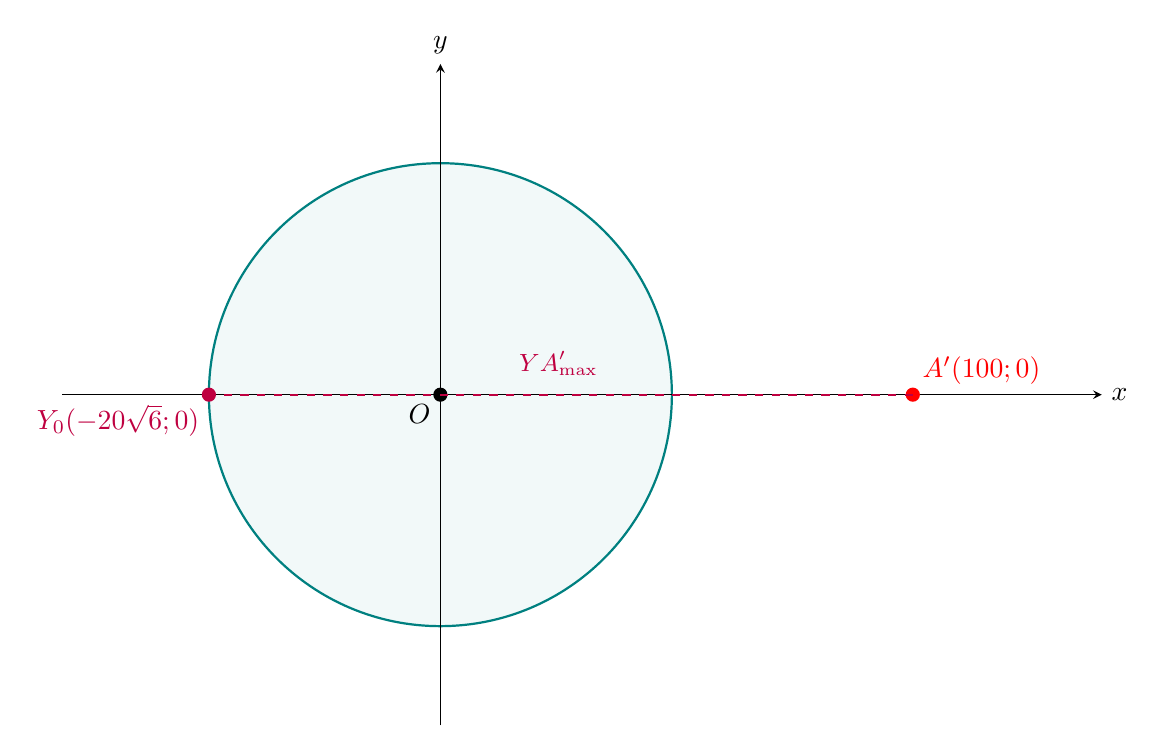
\begin{tikzpicture}[scale=0.06, >=stealth]
				% Đường tròn đáy phẳng trong hệ Oxy
				\fill[teal!5] (0,0) circle (49);
				\draw[thick, teal] (0,0) circle (49);
				\fill[black] (0,0) circle (1.5) node[below left] {$O$};
				
				% Trục tọa độ Oxy phẳng
				\draw[->] (-80,0) -- (140,0) node[right] {$x$};
				\draw[->] (0,-70) -- (0,70) node[above] {$y$};
				
				% Định vị hình chiếu và điểm cực viễn
				\coordinate (Apt) at (100,0);
				\coordinate (Y0) at (-49,0);
				
				\fill[red] (Apt) circle (1.5) node[above right] {$A'(100;0)$};
				\fill[purple] (Y0) circle (1.5) node[below left] {$Y_0(-20\sqrt{6};0)$};
				
				\draw[purple, thick, dashed] (Apt) -- (Y0);
				\node[purple, font=\small, anchor=south] at (25, 2) {$YA_{\max}'$};
			\end{tikzpicture}
		\end{center}
		Giá trị bình phương khoảng cách lớn nhất từ $A$ đến đường tròn là
		$$YA_{\max}^2 = 18800 - 200 \cdot (-20\sqrt{6}) = 18800 + 4000\sqrt{6}$$
		$$\implies YA_{\max} = \sqrt{18800 + 4000\sqrt{6}} \approx 169,1093 \text{ cm}$$
		Vậy khoảng cách tối đa có thể đạt được giữa hai vật $X$ và $Y$ là
		$$XY_{\max} = YA_{\max} + 20 = \sqrt{18800 + 4000\sqrt{6}} + 20 \approx 189\text{ cm}.$$
	}
\end{ex}